\section{Konzeptüberblick} \label{sec:Konzeptüberblick}

Um die Auswirkungen der prädiktiven und reaktiven Ansätze für das \ac{mrcpsp} auf Basis von metaheuristischen Algorithmen bei der Erstellung von Zeitplänen in Bezug auf die Projektdauer bei Verspätungen untersuchen zu können, ist eine Implementierung einer Simulationsumgebung unabdingbar. Diese Umgebung wird im Rahmen der Arbeit als \ac{mrcpsp} Framework bezeichnet. \\

Diese Umgebung muss zunächst in der Lage sein, Zeitpläne für das MRCPSP anhand von Aktivitäts- und Moduslisten (vgl. Abschnitt \ref{subsec:SGS_Aktivitaeten} und Abschnitt \ref{subsec:SGS_Modi}) erstellen zu können. Des Weiteren gilt es mittels Metaheuristiken (vgl. Abschnitt \ref{sec:Metaheuristiken}) gute Zeitpläne im Bezug auf die minimale Projektdauer des \ac{mrcpsp} zu finden. Dennoch bauen prädiktive Verfahren auf eine weitere Metrik auf, nämlich der Robustheit (vgl. Abschnitt \ref{subsec:Praediktive_Methoden}). Somit müssen Metaheuristiken in der Lage sein, Pläne mit der minimalsten Projektdauer zu finden, welche die maximalste Robustheit aufweisen. Das Problem des Findens von Lösungen mit mehreren Zielfunktionen bezeichnet sich als Multi-Objective \cite[vgl. ][S. 146 f.]{abbasi_bi-objective_2006}. Metaheuristiken müssen somit in der Lage sein, Zeitpläne anhand mehrerer Zielfunktionen auswählen zu können. Um zunächst die Performanz der Metaheuristiken unabhängig der Unsicherheitsszenarien vergleichen zu können, muss eine Experimentumgebung geschaffen werden. Diese vergleicht quantitativ die implementierten Metaheuristiken miteinander. \\

Des Weiteren muss eine weitere Experimentumgebung für die Unsicherheitsszenarien realisiert werden. Zunächst gilt es die Unsicherheitsszenarien zu definieren, mit welchen die einzelnen Verfahren innerhalb des Experimentes konfrontiert werden müssen. Es müssen zudem die pro-, prä- und reaktiven Verfahren ausgewählt werden. \\

Die Experimente gilt es auf Benchmark-Instanzen anzuwenden. Hierfür müssen diese Instanzen zunächst ausgewählt und innerhalb des Frameworks hereingeladen werden können.\\

\begin{figure}[H]
    \centering
    \noindent\makebox[\textwidth]{%
    \includegraphics[width=0.70\textwidth]{assets/img/03_Konzept/Konzeptüberblick.drawio.png}
    }
    \caption{Statischer Konzeptüberblick des MRPCSP-Framework} 
    \label{img:mrcpsp_framework}
    \source{Eigene Darstellung}
\end{figure}

Die definierten Anforderungen des MRCPSP Frameworks lassen sich über die Abbildung \ref{img:mrcpsp_framework} visualisieren. Um das MRPCSP Framework zu realisieren wird als Programmiersprache Java ausgewählt. Unterstützend dazu wird das Spring Framework eingesetzt. \\

Bei der populären Programmiersprache Java stehen objektorientierte Programmierung, einfache Wartbarkeit komplexer Software und die Plattformunabhängigkeit durch die Java Virtual Environment im Vordergrund. C bietet als hardwarenahe Sprache dennoch den Vorteil der hohen Geschwindigkeit gegenüber Java. Der Nachteil von manueller Adressverwaltung und somit einer schwierigen Wartbarkeit komplexer Software macht den Vorteil jedoch wett. \cite[vgl.][]{zang_executive_2019}\\

Ein für Java entwickeltes leichtgewichtiges Open Source-Framework stellt Spring dar. Dieses erweitert Java mit dem Dependency Injection-Pattern, was unter anderem leicht entkoppelte Systemkomponenten ermöglicht. Insbesondere für Unternehmen findet Spring in Webanwendungen eine hohe Beliebtheit. Im Rahmen der Masterarbeit wird Spring für die Wartbarkeit und die Auswechselbarkeit von bestimmten Komponenten genutzt, um so den repetitiven Code zu minimieren. \cite[vgl.][]{augsten_was_2019} \\

Insgesamt lässt sich anhand des statischen Konzeptes für das MRCPSP-Framework ein Ablaufplan zur Beantwortung der Forschungsfrage herleiten. Dieser ist in Abbildung \ref{img:mrcpsp_framework_dynamic} aufgezeigt. An vielen Aspekten, wie der Selektion und Konzeption der Lösungs-verfahren, der Auswahl und Integrierung der Benchmarks oder der Generierung der Unsicherheitsszenarien kann unabhängig voneinander entwickelt werden. Erst die Experimente nutzen die verschiedenen Teilaspekte, um so die Güte der einzelnen Methoden und Verfahren quantitativ zu messen. Bei einem Experiment werden die Lösungsverfahren für jede Benchmark-Instanz durchlaufen. Zudem werden bei den Unsicherheitsexperimenten die generierten Unsicherheitsszenarien angewendet. Die Ergebnisse, wie die Makespan-Werte der Basis- und Verspätungszeitpläne werden innerhalb einer CSV-Datei gesammelt. Diese gilt es im Anschluss gemäß der Forschungsfrage zu evaluieren und werden detaillierter im Abschnitt \ref{sec:Experimente} beschrieben. 

\begin{figure}[H]
    \centering
    \noindent\makebox[\textwidth]{%
    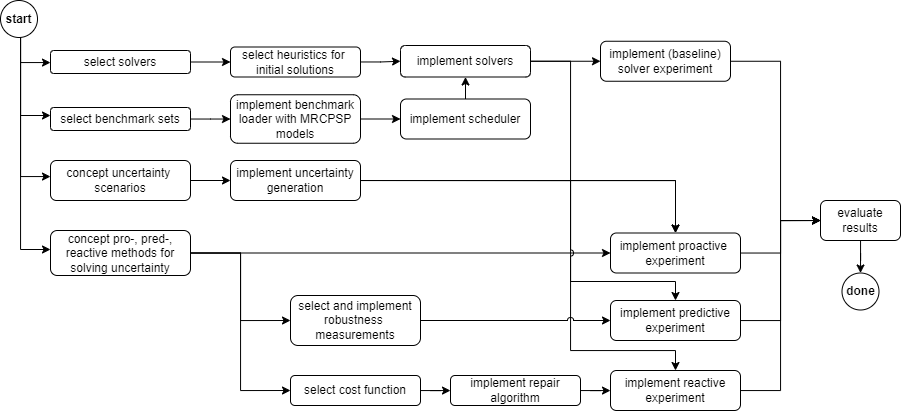
\includegraphics[width=0.91\textwidth]{assets/img/03_Konzept/DynamicConcept.drawio.png}
    }
    \caption{Ablaufplan zur Beantwortung der Forschungsfrage} 
    \label{img:mrcpsp_framework_dynamic}
    \source{Eigene Darstellung}
\end{figure}

% Bei dieser Arbeit gilt es, die im Forschungsfeld etablierten prädiktiven und reaktiven Ansätze auf Basis von metaheuristischen Verfahren für das MRCPSP zu vergleichen. Diese werden auf Benchmarks angewandt, um so die Verfahren auf ein gemeinsames Beispiel vergleichen zu können. Diese Benchmarks müssen im Rahmen der Masterarbeit zunächst ausgewählt und für die Problemstellung aufbereitet werden. Hierfür müssen Unsicherheitsszenarien, wie die Verlängerung von Aufgaben oder Ausfall von Ressourcen in den Benchmarks integriert werden. \\

% Des Weiteren müssen konkrete prädiktive und reaktive Ansätze selektiert werden. Seitens der neu zu implementierenden metaheuristischen Ansätzen wird der Fokus auf evolutionäre Algorithmen, Tabu Search, Simulated Annealing.\\

% Die zu untersuchenden Ansätze werden innerhalb eines Frameworks in der Programmiersprache Java implementiert. Dieses ermöglicht zudem den Import der Bench-mark-Instanzen, berechnet Zeitpläne und übernimmt die Messung der gewünschten Werte, wie die Robustheit und Durchlaufdauer. Im Anschluss gilt es diese Werte über die zu untersuchenden Ansätze miteinander zu vergleichen, um daraus die Forschungsfrage und dessen Unterfragen beantworten zu können. 


% Auswahl von Benchmarks
% Auswahl von Metaheuristiken
% Auswahl von prädiktiven- prediktive und proaktiven Verfahren